% Section 2.2: the PPO agent, the belief encoder side network and the training pipeline.
% Build: tectonic architecture.tex  (standalone, drawn at full text width, about 5.5 in)
% Sources: figgie/rl/policy.py (ActorCritic, arch gru), figgie/rl/features.py (16 per-suit inputs),
% figgie/rl/train.py (BC from Bayesian, PPO with PFSP), scripts/train_encoder.py (belief encoder).
\PassOptionsToPackage{table}{xcolor}
\documentclass[tikz,border=1pt]{standalone}
\usepackage[T1]{fontenc}
\usepackage[scaled=0.95]{helvet}
\renewcommand{\familydefault}{\sfdefault}
\usetikzlibrary{positioning,arrows.meta,calc,fit,backgrounds}

\definecolor{blue}{HTML}{0072B2}
\definecolor{verm}{HTML}{D55E00}
\definecolor{grey}{HTML}{666666}
\definecolor{ink}{HTML}{222222}
\definecolor{green}{HTML}{009E73}
\definecolor{orange}{HTML}{E69F00}

% small second-line detail inside a box
\newcommand{\sub}[1]{{\fontsize{6.8}{7.9}\selectfont\color{ink!85}\begin{tabular}{@{}c@{}}#1\end{tabular}}}

% a short strip of example values in small monospace cells, Transformer-diagram style
\usepackage{pifont}
\newcommand{\cells}[2]{{\ttfamily\fontsize{5.6}{6.4}\selectfont\setlength{\tabcolsep}{1.5pt}%
  \renewcommand{\arraystretch}{1.05}\arrayrulecolor{#1!70}\begin{tabular}{|*{12}{c|}}\hline\rowcolor{white}#2\\\hline\end{tabular}}}
\newcommand{\red}[1]{\textcolor{red!75!black}{#1}}
\begin{document}
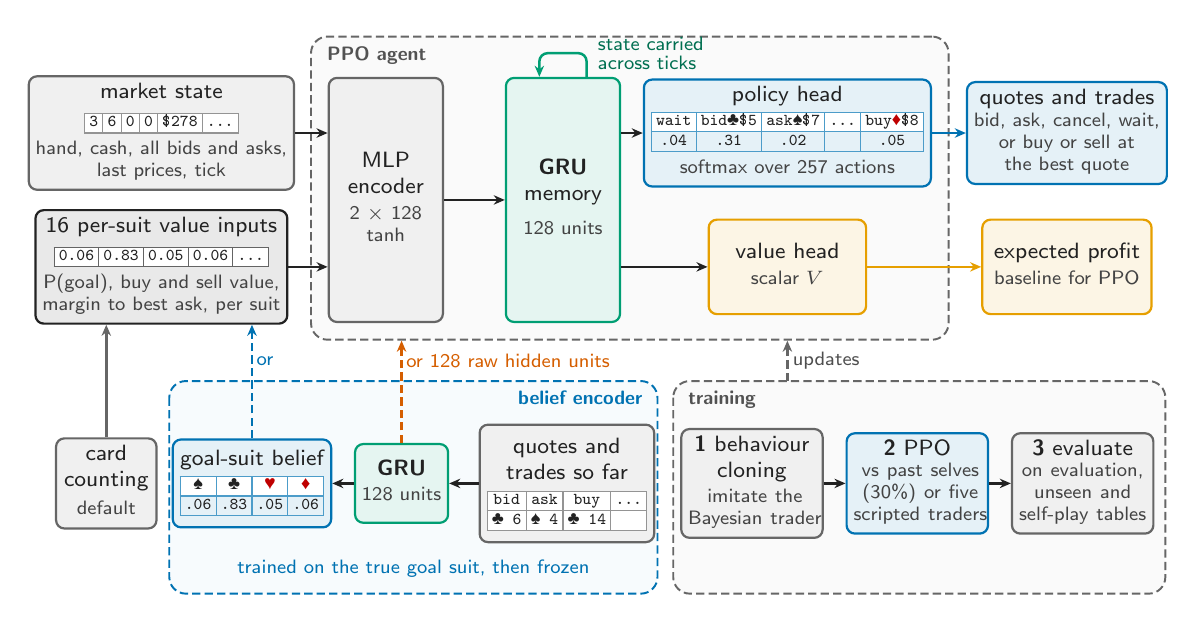
\begin{tikzpicture}[
    font=\fontsize{8}{9.4}\selectfont,
    >={Stealth[length=4pt,width=3.4pt]},
    box/.style={draw=#1, fill=#1!10, rounded corners=3pt, line width=0.8pt,
                align=center, inner sep=2.5pt, text=ink},
    small/.style={font=\fontsize{6.8}{7.9}\selectfont, text=ink!80},
    flow/.style={->, line width=0.9pt, draw=#1, rounded corners=3pt},
    group/.style={draw=#1, rounded corners=6pt, line width=0.7pt, dash pattern=on 3pt off 1.5pt, fill=#1!3},
    tag/.style={font=\fontsize{7.5}{8.5}\selectfont\bfseries, text=#1, inner sep=1pt},
  ]
  % =============================================================== agent
  \node[box=grey, minimum width=2.7cm, minimum height=1.4cm] (mkt) at (1.35,-0.8)
       {market state\\[1pt]\cells{grey}{3&6&0&0&\$278&\ldots}\\[1pt]\sub{hand, cash, all bids and asks,\\last prices, tick}};
  \node[box=ink, minimum width=2.7cm, minimum height=1.4cm] (psv) at (1.35,-2.5)
       {16 per-suit value inputs\\[1pt]\cells{ink}{0.06&0.83&0.05&0.06&\ldots}\\[1pt]\sub{P(goal), buy and sell value,\\margin to best ask, per suit}};

  \node[box=grey, minimum width=1.45cm, minimum height=3.1cm] (mlp) at (4.2,-1.65)
       {MLP\\encoder\\[3pt]\sub{2 $\times$ 128\\tanh}};
  \node[box=green, minimum width=1.45cm, minimum height=3.1cm] (gru) at (6.45,-1.65)
       {\textbf{GRU}\\memory\\[3pt]\sub{128 units}};
  \node[box=blue, minimum width=2.0cm, minimum height=1.2cm] (pi) at (9.3,-0.8)
       {policy head\\[1pt]\cells{blue}{wait&bid\ding{168}\$5&ask\ding{171}\$7&\ldots&buy\red{\ding{169}}\$8\\\hline .04&.31&.02&&.05}\\[1pt]\sub{softmax over 257 actions}};
  \node[box=orange, minimum width=2.0cm, minimum height=1.2cm] (vf) at (9.3,-2.5)
       {value head\\\sub{scalar $V$}};
  \node[box=blue, minimum width=2.15cm, minimum height=1.2cm] (act) at (12.85,-0.8)
       {quotes and trades\\\sub{bid, ask, cancel, wait,\\or buy or sell at\\the best quote}};
  \node[box=orange, minimum width=2.15cm, minimum height=1.2cm] (val) at (12.85,-2.5)
       {expected profit\\\sub{baseline for PPO}};

  \draw[flow=ink] (mkt.east) -- (mkt.east -| mlp.west);
  \draw[flow=ink] (psv.east) -- (psv.east -| mlp.west);
  \draw[flow=ink] (mlp.east) -- (gru.west);
  \draw[flow=ink] (gru.east |- pi.west) -- (pi.west);
  \draw[flow=ink] (gru.east |- vf.west) -- (vf.west);
  \draw[flow=blue]   (pi.east) -- (act.west);
  \draw[flow=orange] (vf.east) -- (val.west);
  % recurrence h_{t-1} -> h_t
  \draw[flow=green] ($(gru.north)+(0.3,0)$) -- ++(0,0.3) -| ($(gru.north)+(-0.3,0)$);
  \coordinate (looptop) at ($(gru.north)+(0,0.3)$);
  \node[small, text=green!70!black, right=0.32cm of looptop, align=left] {state carried\\[-1pt]across ticks};

  \begin{scope}[on background layer]
    \node[group=grey, fit=(mlp)(gru)(pi)(vf)(looptop), inner xsep=6pt, inner ysep=6pt] (agent) {};
  \end{scope}
  \node[tag=grey!80!black, anchor=north west] at ($(agent.north west)+(5pt,-3pt)$) {PPO agent};

  % =============================================================== bottom row: one shared top and bottom
  \def\rowtop{-3.95}
  \def\rowbot{-6.65}
  \def\rowmid{-5.25}

  % card counting, the default source of the per-suit inputs
  \node[box=grey, text width=1.1cm, minimum height=1.0cm] (cc) at (0.65,\rowmid)
       {card\\counting\\[1pt]\sub{default}};
  \draw[flow=grey] (cc.north) -- (cc.north |- psv.south);

  % belief encoder, a separate supervised network (reads right to left)
  \node[box=blue, minimum height=1.0cm, inner ysep=4pt] (bel) at (2.5,\rowmid)
       {goal-suit belief\\[1pt]\cells{blue}{\ding{171}&\ding{168}&\red{\ding{170}}&\red{\ding{169}}\\\hline .06&.83&.05&.06}};
  \node[box=green, minimum width=1.1cm, minimum height=1.0cm] (egru) at (4.4,\rowmid)
       {\textbf{GRU}\\\sub{128 units}};
  \node[box=grey, minimum height=1.0cm, inner ysep=4pt] (eobs) at (6.5,\rowmid)
       {\begin{tabular}{@{}c@{}}quotes and\\trades so far\\[1pt]\cells{grey}{bid&ask&buy&\ldots\\\hline \ding{168} 6&\ding{171} 4&\ding{168} 14&}\end{tabular}};
  \draw[flow=ink] (eobs.west) -- (egru.east);
  \draw[flow=ink] (egru.west) -- (bel.east);
  \node[small, text=blue, align=center, anchor=south] (enccap) at (4.55,\rowbot+0.08)
       {trained on the true goal suit, then frozen};
  \begin{scope}[on background layer]
    \draw[group=blue] (1.45,\rowtop) rectangle (7.65,\rowbot);
  \end{scope}
  \node[tag=blue, anchor=north east] at (7.65-0.15,\rowtop-0.08) {belief encoder};

  \draw[flow=blue, dash pattern=on 3pt off 1.5pt] (bel.north) -- (bel.north |- psv.south);
  % right of the arrow, level with the orange label
  \node[small, text=blue, anchor=west, inner sep=1.5pt] at ($(bel.north |- agent.south)!0.5!(bel.north |- 0,\rowtop)$) {or};
  \draw[flow=verm, dash pattern=on 3pt off 1.5pt] (egru.north) -- (egru.north |- agent.south);
  % one-line label right of the arrow, in the gap between the agent and the encoder
  \node[small, text=verm, anchor=west, inner sep=1.5pt] at ($(egru.north |- agent.south)!0.5!(egru.north |- 0,\rowtop)$)
       {or 128 raw hidden units};

  % =============================================================== training pipeline
  \node[box=grey, text width=1.62cm, minimum height=1.25cm] (bc) at (8.85,\rowmid)
       {\textbf{1} behaviour\\cloning\\[1pt]\sub{imitate the\\Bayesian trader}};
  \node[box=blue, text width=1.62cm, minimum height=1.25cm] (ppo) at (10.95,\rowmid)
       {\textbf{2} PPO\\[1pt]\sub{vs past selves\\(30\%) or five\\scripted traders}};
  \node[box=grey, text width=1.62cm, minimum height=1.25cm] (ev) at (13.05,\rowmid)
       {\textbf{3} evaluate\\[1pt]\sub{on evaluation,\\unseen and\\self-play tables}};
  \draw[flow=ink] (bc.east) -- (ppo.west);
  \draw[flow=ink] (ppo.east) -- (ev.west);
  \begin{scope}[on background layer]
    \draw[group=grey] (7.85,\rowtop) rectangle (14.1,\rowbot);
  \end{scope}
  \coordinate (train) at (7.85,\rowtop);
  \node[tag=grey!80!black, anchor=north west] at (7.85+0.15,\rowtop-0.08) {training};
  \draw[flow=grey, dash pattern=on 3pt off 1.5pt] (vf.south |- train) -- (vf.south |- agent.south)
       node[pos=0.5, right, small, inner sep=1.5pt] {updates};
\end{tikzpicture}
\end{document}
